\section{Lens Hood Model: Additional Count Rate from Arbitrary Source}
Let $s(\theta)$ be the lens hood suppression as a function of angle $\theta$ 
from the camera boresight to a given point-source on the sky. By definition,
\begin{equation}
s(\theta) \equiv \frac{F_\mathrm{obs}}{F_\mathrm{ns}},
\end{equation}
for $F_\mathrm{obs}$ the observed flux of the source (that which reaches the 
CCD), and $F_\mathrm{ns}$ the flux that would be observed with no 
suppression and $\theta=0$.
The observed flux of the source can then be written as a function of $\theta$
\begin{align}
	F_\mathrm{obs}(\theta) &= s(\theta) F_\mathrm{ns}  \\
	&= s(\theta) F_0 10^{-0.4(m_\mathrm{ns} - m_0)} ,
\end{align}
for $F_0$ the (non-suppressed) flux corresponding to a source with zero-point 
apparent magnitude $m_0$, and $m_\mathrm{ns}$ the apparent magnitude of 
the source with no suppression.
\citet{winn_searchable_2013} tabulates $F_0 = 
1.6\times10^6\,\mathrm{ph/s/cm^2}$ 
for an $I=0$, G2V star.
Thus
\begin{equation}
F_\mathrm{obs}(\theta) = (1.6\times 10^6) s(\theta) 10^{-0.4 m_\mathrm{ns}} 
\quad \mathrm{[ph/s/cm^2]}.
\end{equation}

We can then write the following expression for $\mu\equiv F_\mathrm{obs} A \eta 
/ N$, the mean incident count rate on the pixel of interest:
\begin{equation}
\mu =  (1.6\times 10^6) s(\theta) 10^{-0.4 m_\mathrm{ns}} \frac{A 
\eta}{N} \quad \mathrm{[ct/px/s]},
\end{equation}
for $A$ the effective observing area in $\mathrm{cm^2}$, $N$ the 
number of pixels per camera, and $\eta$ the quantum efficiency.
For TESS, $A=69.1\,\mathrm{cm^2}$, $N=4096^2$, and $\eta\approx 1$. Using
these numbers gives
\begin{equation}
\mu = 6.59  s(\theta) 10^{-0.4 m_\mathrm{ns}}\quad 
\mathrm{[ct/px/s]}.
\label{eq:mean_added_flux}
\end{equation}
Assuming a Poisson arrival rate, the standard deviation in the number of counts 
per pixel per 2 second readout is then
\begin{equation}
\sigma \approx \mu^{1/2} = \left[ 13.2 s(\theta) 10^{-0.4 m_\mathrm{ns}} 
\right]^{1/2}\quad \mathrm{[ct/px\ RMS\ per\ 2\ sec\ image]}.
\label{eq:added_RMS}
\end{equation}

The above expression assumes that the scattered flux from the source 
is uniformly spread across the CCD. The reality may be quite different,
but our purpose in this case is to simply get order-of-magnitude accuracy.
Another caveat is that our zero-point relies on an $I$ magnitude calibration -- 
a more accurate approach would use separate bandpass-dependent zero-points.

To compute the net effect on TESS's noise budget, we add $\sigma$ from 
Eq.~\ref{eq:added_RMS} in quadrature with Eq.~\ref{eq:snr}.
We assume $m_\mathrm{ns}$ values of $-26,-13,\,\mathrm{and}\ -17.76$ for the 
Sun, Moon, and Earth respectively.
This gives Figs.~\ref{fig:sun_scat}-\ref{fig:earth_scat}.

\begin{figure}[!h]
	\centering
	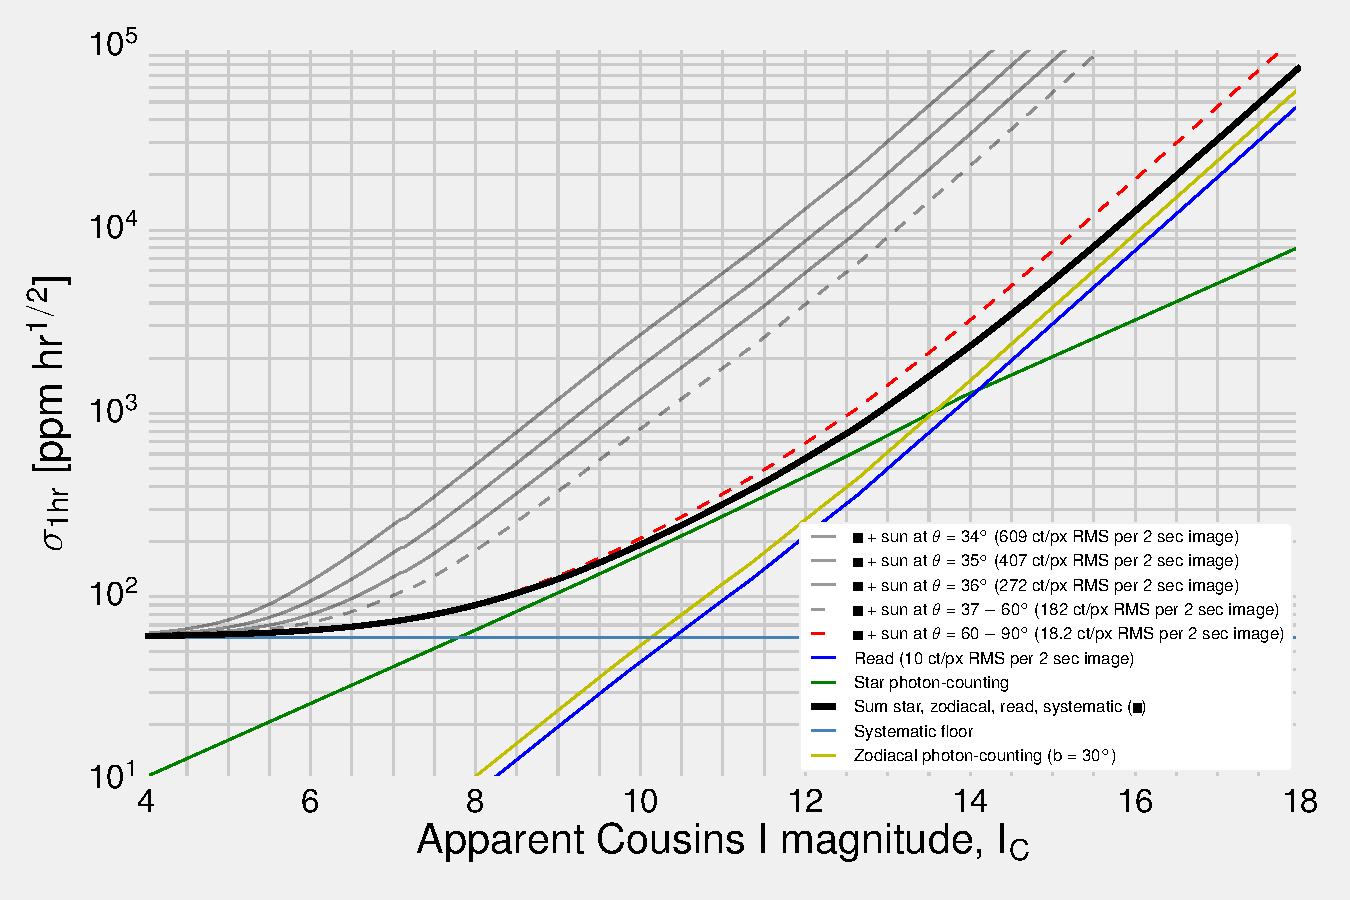
\includegraphics{figures/precision_angles_sun.pdf}
	\caption{Noise budget including Solar scattered light at different angles 
		$\theta$ from camera boresight. 
		Note that the suppression model 
		(Fig.~\protect\ref{fig:lens_hood_suppression}) 
		accounts solely for lens hood suppression, omitting sunshade 
		suppression (which substantially lowers the dashed red line for most
		orientations of the Sun).
		The number given in brackets is $\sigma$ in 
		Eq.~\protect\ref{eq:added_RMS} --
		the extra standard deviation about the mean.
		Squaring, lines where $\mu \gtrsim 10^5 \mathrm{ct/px/s}$ will saturate 
		the CCD pixels (and thus are not plotted).} 
	\label{fig:sun_scat}
\end{figure}
\begin{figure}[!h]
	\centering
	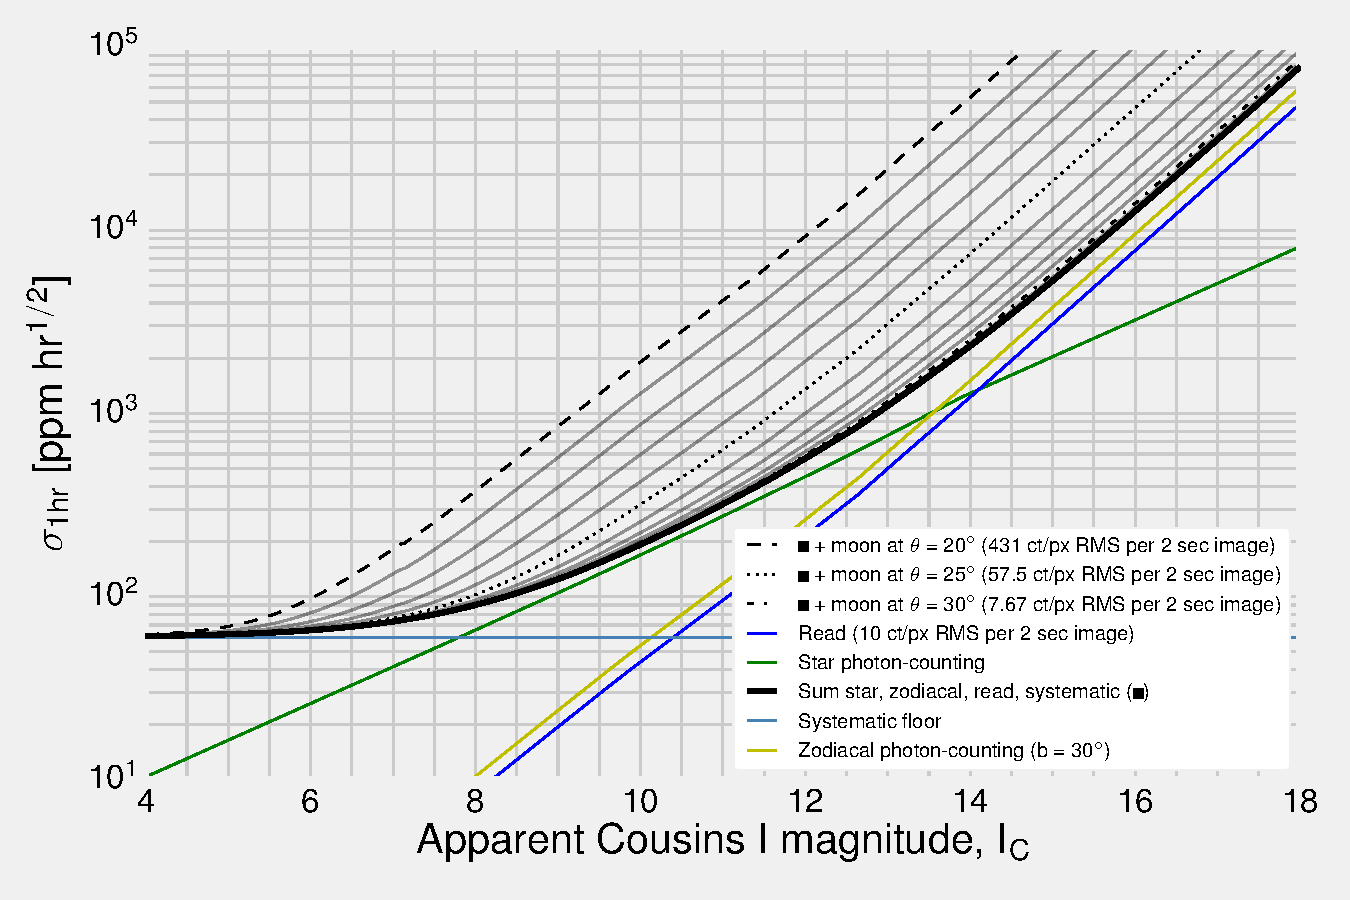
\includegraphics{figures/precision_angles_moon.pdf}
	\caption{Same as Fig.~\protect\ref{fig:sun_scat}, for scattered Moonlight.
		Gray lines are spaced by $1^\circ$.} 
	\label{fig:moon_scat}
\end{figure}
\begin{figure}[!h]
	\centering
	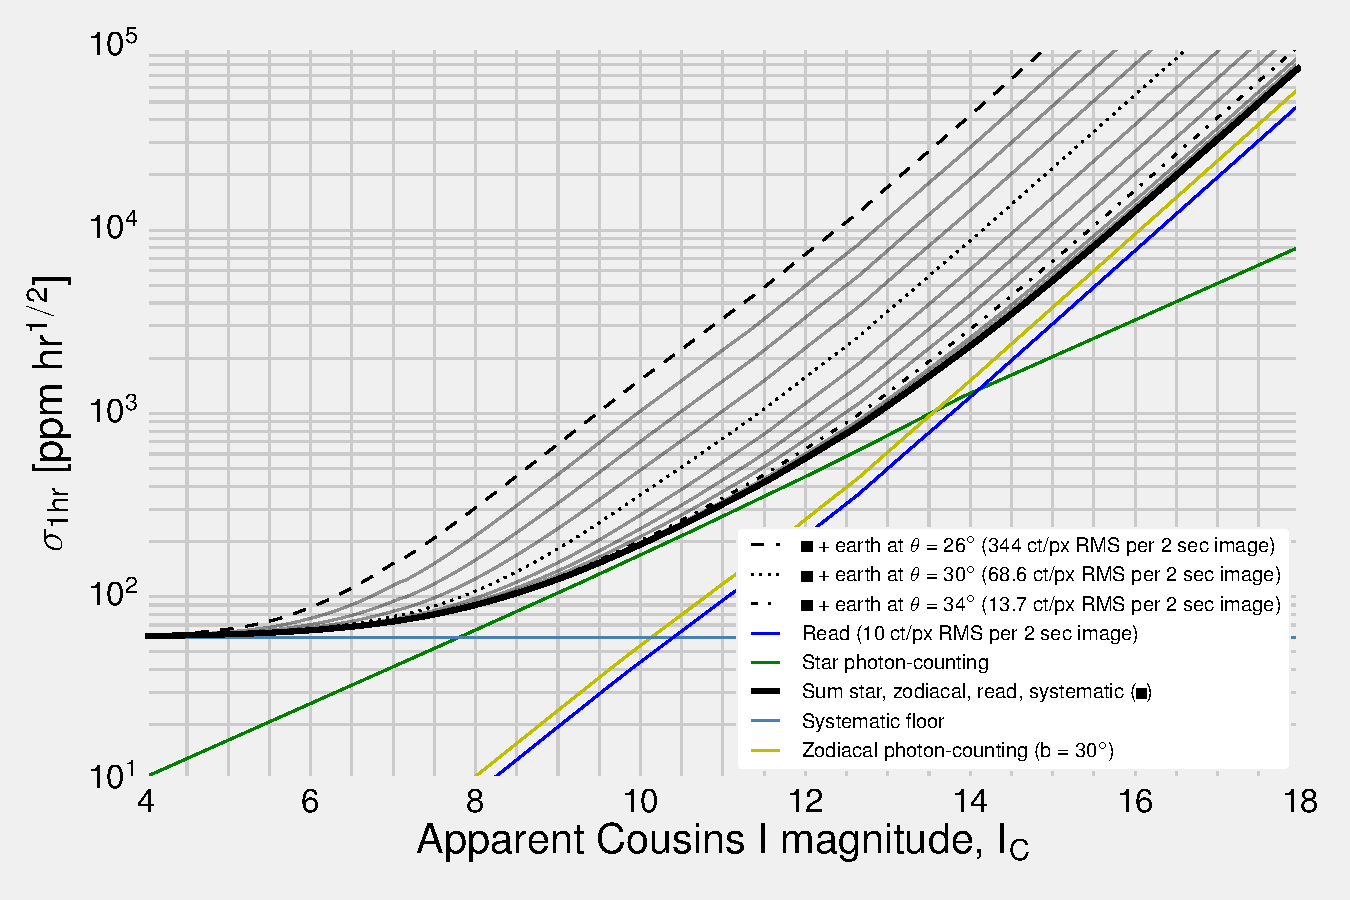
\includegraphics{figures/precision_angles_earth.pdf}
	\caption{Same as Fig.~\protect\ref{fig:sun_scat}, for scattered 
		Earthlight. Gray lines are spaced by $1^\circ$.} 
	\label{fig:earth_scat}
\end{figure}

 

